\chapter{FreshSolution:清新の试题解析模板}
\centerline{Xia Mingyu, Hangzhou Dianzi University}

\centerline{\today, Version 0.1a}
\section{FreshSolution模板简介}
{
\color{Periwinkle}FreshSolution模板致力于打造一系列清新、淡雅的模板,用于各大高校排版高等数学、大学物理或其他专业课的试题解析.本文将介绍本模板的一些设置内容以及基本使用方法.如果您有其他问题,建议或者意见,欢迎在 GitHub 上提交 issues 或者邮件联络,共享您的ideas.

本模板基于Elegant\LaTeX 开发,标题背景的设计思路参考了VividBook的设计方案,在此对两个模板作者先前的工作表示感谢.

此模板原为本人为所在学校的公共基础课制作《大学物理》的历年试题解析的文档,最初使用Elegant\LaTeX 排版,后根据本人需要做出诸多调整,最终发展到了现在的解析模板.当然,这是此模板「出道」的第一个版本,还存在诸多不足与功能的缺失,望大家多多提出宝贵的意见与建议.

作者的联系方式如下,建议加入用户 QQ 群提问,这样能更快获得准确的反馈.

\begin{multicols}{2}

    \faEnvelope\ \email{xiamyphys@gmail.com}
    
    \faQq\ \href{https://qm.qq.com/cgi-bin/qm/qr?k=gg5GsqSkGvZbC6TphVMlXRl08vqMV9Lw&authKey=rDcxqMdHwxWLQQBZwgfHduopCmVulM8CTWUhsGFOWyjqo6Ekk0omdoi4kuzxC/k4&noverify=0}{760570712}

    \faGithub\ \href{https://github.com/xiamyphys/FreshSolution.git}{https://github.com/sxiamyphy/FreshSolution.git}

    \faWechat\ \href{http://weixin.qq.com/r/hR1SSofEIdpercMp90iX}{物理問題作}
\end{multicols}

\newpage
\begin{multicols}{2}
\section{关于作者}
\bfseries
    \begin{itemize}
        \item 钱江北岸某不知名高校光电专业大三在读生
        \item 60\%物理+30\%数学+9\%骑行圈+1\%\LaTeX
        \item 土生土长的东北银儿,开口说话苞米碴子味~
        \item ?闲没事喜欢哼上一首Ado的歌
        \item $\cdots$
    \end{itemize}
    \newcolumn
    \begin{center}
        \vspace{1em}
        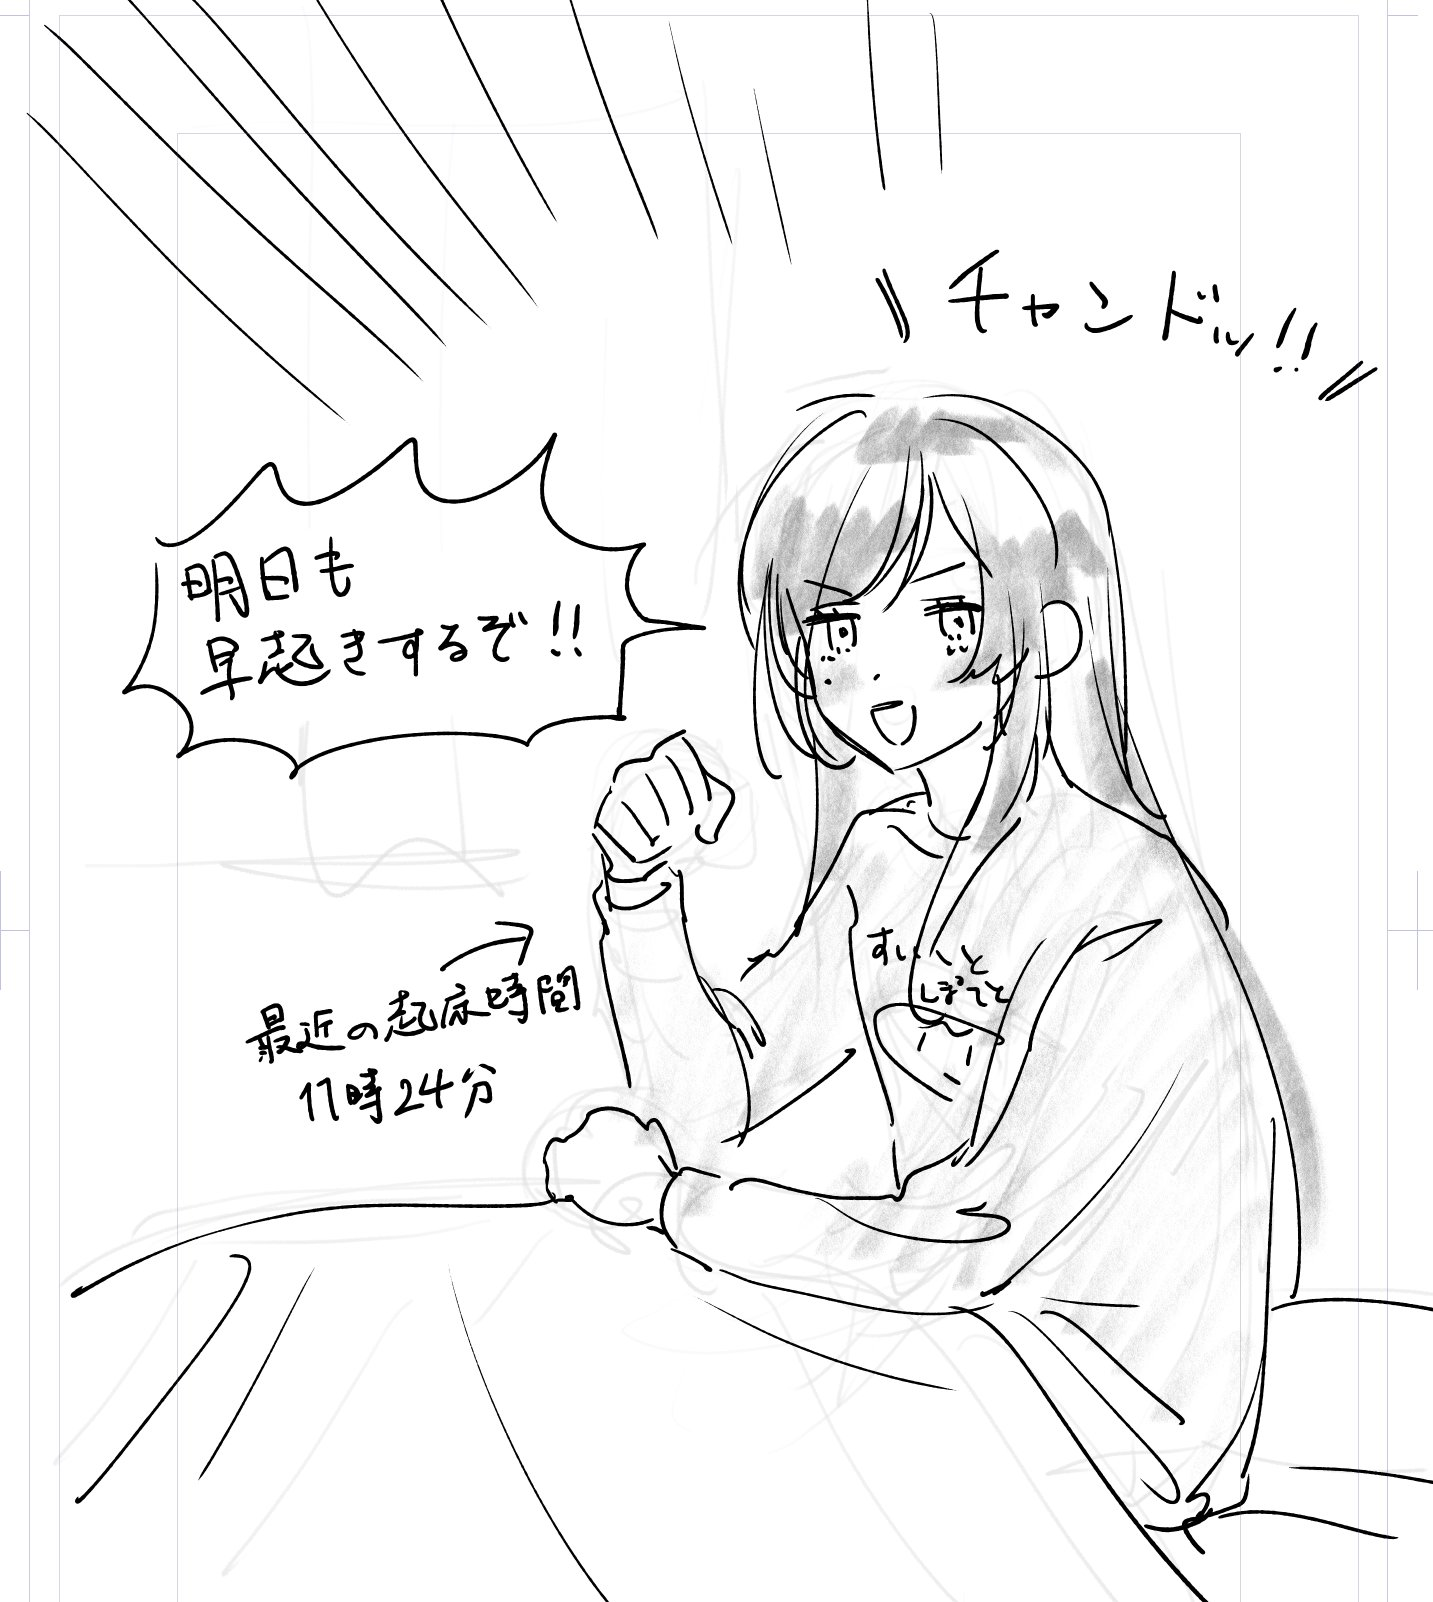
\includegraphics[width=0.32\textwidth]{introduction.JPG}
    \end{center}
\end{multicols}
\newpage
\section{模板内容介绍}
\subsection{章节标题背景设置}
在FreshSolution.tex文件中使用chapterimage命令后,其后方所有input命令插入的cha文件夹中各章节的tex的标题背景将都是此背景,直至下一个chapterimage出现才会变为新的背景,以此类推.

\subsection{解析设置}
本模板提供两种解析模式,分别为 answer=ans 和 answer=noans,默认选项为ans。在启动noans模式后,将掩盖解答Solution环境中所有的内容,便于用户导出无解析的试题.

为提高效率,针对选择题解析增加命令\verb|\sokka{}|(sokka是日语「そっか」的罗马音,意思是“原来如此”),变量内填写对应字母,就会输出“故本题选择\{\}项.”如\verb|\sokka{B}|输出为“\sokka{B}”
\begin{tcblisting}{}
\begin{solution}
由高斯定理,通过$S$面的电通量为$\frac{q}{\varepsilon_0}$;$S$面上各点的场强由$+q$和$-q$所激发.\sokka{D}
\end{solution}
\end{tcblisting}
\subsection{选择题环境}
选择题环境共包含两个选项,第一个为本题答案,第二个为本题考点,代码示例如下所示.
\begin{tcblisting}{sidebyside}
    \begin{choice}{D}{高斯定理}
        这是题目.
        \begin{tasks}(2)% (2)表示每行两个选项
            \task 这是A选项
            \task 这是B选项
            \task 这是C选项
            \task 这是D选项
        \end{tasks}
    \end{choice}
\end{tcblisting}

\hspace{-2.16em}
\begin{minipage}{0.67\textwidth}
\vspace{1em}
\begin{choice}{D}{高斯定理}
    $A$和$B$为两个均匀带电球体,$A$带电荷$+q$,$B$带电荷$-q$,作一与$A$同心的球面$S$为高斯面,如图所示.则
    \begin{tasks}
        \task 通过$S$面的电场强度通量为零,$S$面上各点的场强为零.
        \task 通过$S$面的电场强度通量为$\frac{q}{\varepsilon_0}$,$S$面上各点的场强为$E=\frac{q}{4\pi\varepsilon_0r}$b
        \task 通过$S$面的电场强度通量为$-\frac{q}{\varepsilon_0}$,$S$面上各点的场强为$E=\frac{q}{4\pi\varepsilon_0r}$
        \task 通过$S$面的电场强度通量为$\frac{q}{\varepsilon_0}$,但是$S$面上各点的场强不能直接由高斯定理求出.
    \end{tasks}
\end{choice}
\end{minipage}
\hfill
\begin{minipage}[c]{0.33\textwidth}
\begin{center}
    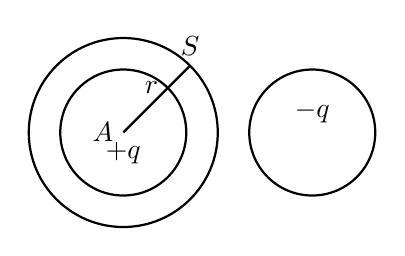
\begin{tikzpicture}
    \draw [thick] (0,0) circle (0.8);
    \draw [thick] (0,0) circle (1.2);
    \draw [thick] (2.4,0) circle (0.8);
    \draw [thick] (0,0)--(0.85,0.85);
    \node [anchor=east] at (0,0) {$A$};
    \node [anchor=north] at (0,0) {$+q$};
    \node [anchor=east] at (0.566,0.566) {$r$};
    \node [anchor=south] at (0.85,0.85) {$S$};
    \node [anchor=south] at (2.4,0) {$-q$};
    \end{tikzpicture}
\end{center}
\end{minipage}

\subsection{试题环境}
与选择题环境有少许不同,两个选项分别为分数与考点,题号计数器和选择题共用,代码示例如下所示.
\begin{tcblisting}{sidebyside}
    \begin{exercise}{5}{考点1,考点2,……}
        这是试题.
    \end{exercise}
\end{tcblisting}
    \hspace{-2.16em}
    \begin{minipage}{0.67\textwidth}
        \vspace{1em}
    \begin{exercise}{6}{高斯定理,场强计算}
        一均匀带电直导线长为$d$,电荷线密度为$+\lambda$.过导线中点$O$作一半径为$R$($R>\frac{d}{2}$)的球面$S$,$P$为带电直导线的延长线与球面$S$的交点.则通过该球面的电场强度通量$\Phi_e=$\ans{$\frac{\lambda d}{\varepsilon_0}$},带电直线的延长线与球面交点$P$处的电场强度的大小为\ans{$\frac{\lambda d}{4\pi\varepsilon_0\ab(R^2-d^2/4)}$},方向\ans{沿矢径$\boldsymbol{OP}$}.
    \end{exercise}
    \end{minipage}
    \hfill
    \begin{minipage}[c]{0.33\textwidth}
    \begin{center}
        \begin{tikzpicture}[scale=0.83]
        \draw (0,0) circle (2);
        \draw [thick,->] (-2,0)--(0,0)--(1,1.732);
        \node [anchor=east] at (-2,0) {$P$};
        \filldraw (-2,0) circle (0.05);
        \node [anchor=west] at (0.5,0.866) {$R$};
        \filldraw [pattern=north east lines] (-0.8,-0.1)--(-0.8,0.1)--(0.8,0.1)--(0.8,-0.1)--cycle;
        \draw [thick,|<-] (-0.8,-0.3)--(-0.25,-0.3);
        \draw [thick,|<-] (0.8,-0.3)--(0.25,-0.3);
        \node at (0,-0.3) {$L$};
        \end{tikzpicture}
    \end{center}
    \end{minipage}

\subsection{字体设置}
本模板全局选项中支持mtpro2字体,用户电脑安装该字体后方可使用.
\subsection{页码设置}
全局选项中支持"seperate"与"continuous"两个选项,前者为每章节开始时页码计数器重置为1,后者则页码连续.缺省值为separate.
}
\newpage
\subsection{分栏排版示例}
{
\begin{multicols}{2}
\begin{exercise}{8}{场强计算}
    一半径为$R$的带电球体,其电荷体密度分别为
    $$\left\{
    \begin{aligned}
        &\rho=\frac{qr}{\pi R^4}&&\ab(r\le R)\\
        &\rho=0&&\ab(r>R)
    \end{aligned}\right.
    $$
    其中$q$为一正的常量.试求
    \begin{enumerate}
        \item 带电球体的总电荷;
        \item 球内、外各点的电场强度.
    \end{enumerate}
\end{exercise}
\begin{solution}
    \begin{enumerate}
        \item 
        $$
        \begin{aligned}
            Q&=\iiint{\rho\d V}\\
            &=\int_0^R{\frac{qr}{\pi R^4}4\pi r^2\d r}=q
        \end{aligned}
        $$
    \end{enumerate}
\end{solution}
\begin{soluting}
    \begin{enumerate}[label=2]
        \item 分别取$r<R$和$r\ge R$的高斯面.
        
        由高斯定理
        $$E\cdot 4\pi r^2=\frac{\displaystyle\int_0^r{\dfrac{qr}{\pi R^4}4\pi r^2\d r}}{\varepsilon_0}$$
        $$E\cdot 4\pi r^2=\frac{q}{\varepsilon_0}$$
        解得
        $$
        E=\left\{
            \begin{aligned}
                &\frac{1}{4\pi\varepsilon_0}\frac{qr^2}{R^4}&& r<R\\
                &\frac{1}{4\pi\varepsilon_0}\frac{q}{r^2}&& r\ge R
            \end{aligned}
        \right.$$
    \end{enumerate}
\end{soluting}
\end{multicols}
}